\documentclass{article}
\usepackage{a4}
\usepackage[utf8]{inputenc}
\usepackage{xspace}
\usepackage{amsmath,amssymb}
\usepackage{tikz}
\newcommand{\DD}{\mathbb D}
\newcommand{\RR}{\mathbb R}
\DeclareMathOperator{\NN}{\mathbb N}
\DeclareMathOperator{\C}{\mathcal C}
\DeclareMathOperator{\laplace}{\Delta}
\DeclareMathOperator{\dom}{\mathrm{dom}}
\bibliographystyle{amsalpha}

\newcommand{\p}{\ensuremath{\mathcal P}\xspace}
\newcommand{\np}{\ensuremath{\mathcal{NP}}\xspace}
\newcommand{\fp}{\ensuremath{\mathcal{FP}}\xspace}
\newcommand{\sharpp}{\ensuremath{\# \mathcal{P}}\xspace}
\newcommand{\cc}{\texttt{C++}\xspace}
\newcommand{\irram}{\texttt{iRRAM}\xspace}
\newcommand{\REAL}{\texttt{REAL}\xspace}
\newcommand{\BA}{\texttt{BASE\_ANA}\xspace}
\newcommand{\AR}{\texttt{ANA\_RECT}\xspace}
\DeclareMathOperator{\CC}{\mathbb C}

\begin{document}
\title{Analytic Functions in \irram\thanks{
Supported in part by \emph{JSPS Kakenhi} projects
\texttt{23700009} and \texttt{24106002},
by \emph{7th EU IRSES} project \texttt{294962},
by \emph{DFG} project \texttt{Zi\,1009/4-1},
and by \emph{DAAD}.}}
\author{Akitoshi Kawamura$^1$, \quad Florian Steinberg$^2$, \quad Holger Thies$^{1,2}$ 
\\
$^1$ The University of Tokyo (JAPAN), \quad $^2$ TU Darmstadt (GERMANY)}
\date{}
\maketitle
\noindent
The Type-2 Theory of Effectivity provides a sound framework for investigating the computability of real numbers, sequences, functions, and operators.
It is well known that an analytic function on a compact domain is computable if and only if its sequence of Taylor coefficients is computable.
However, an algorithm evaluating a given power series must in addition to said coefficient sequence be provided with additional information about its rate of convergence \cite{Mueller95}.
On simple domains, this information can be realized by two integer parameters.
Moreover, Real Complexity Theory shows that this representation renders the usual operations on analytic functions uniformly computable within parameterized polynomial time \cite{Kawamura2012}.
This is in contrast with the situation for smooth functions where maximization has been shown to correspond to the \p vs. \np Millennium Prize Problem \cite{MR666209} and integration to the even stronger \fp vs. \sharpp question \cite{MR748898,MR1137517}.
Theory thus suggests a mixed real/integer data structure and interface declaration for practical and efficient implementations of power series in imperative programming.
\irram constitutes a free library to build upon, conveniently providing an abstract data type \REAL in \cc.

We present such a prototype implementation of power series and analytic functions on a fixed line segment.
The data type encodes a germ enriched with integer information as described above;
it supports basic operations like pointwise addition and multiplication, composition, differentiation and integration.
Evaluation is realized by analytic continuation using iterated evaluation and interpolation.
We proceed to explore the practical performance of our implemented and compare its empirical behaviour with the theoretical predictions.

\bigskip

Let $\DD$ denote the closed complex unit disc.
The analytic functions on $\DD$ are in one to one correspondence with the sequences $\overline a = (a_n)_{n\in \NN}$, whose radius of convergence is strictly larger than $1$ via the assignment
\[ \overline a \mapsto f_{\overline a}, \quad\text{where}\quad f_{\overline a}(x)= \sum_{n\in \NN} a_n x^n, \]
resp.
\[ f \mapsto \left(\frac{f^{(n)}(x)}{n!}\right)_{n\in \NN}. \]
These assignments can easily be seen to be discontinuous and therefore not computable.
Thus consider tuples $\big(A,k,(a_n)_{n\in\NN}\big)$, where $A$ and $k$ are integers such that
\begin{itemize}
\item $r:=\sqrt[k]{2}$ is strictly smaller than the radius of convergence of $(a_n)_{n\in \NN}$
\item $|a_n|  r^n \leq A$ for all $n\in \NN$.
\end{itemize}
The evaluation operator $\big(A,k,(a_n)_{n\in \NN},x\big)\mapsto f_{\overline a}(x)$ becomes computable in time polynomial in the binary output precision, in $\log(A)$, and in $k$.
Moreover, addition, integration, maximization and many other basic operations on power series can be shown to be parameterized polynomial time computable if considered as multivalued operators on such tuples.

The data type \BA realizes the above theoretical considerations as an interface class for \irram.
There is an constructor, constructing a \BA object from a given power series together with integers $A$ and $k$, where the user has to make sure they fulfill the above relations.
The standard operators $+$, $*$ are overloaded to also work for these objects and differentiation as well as integration and evaluation are implemented.

Our implementation of a data type \AR for analytic functions on a line segment follows the ideas from \cite{Kawamura2012} closely.
That is, a function $f$ on a line segment can either be represented by its Taylor sequence around some point $x_0$ on the line segment and integer parameters $A$ and $k$ such that $f^{(j)}(x)\leq A k^j j!$ for all $x$ in the line segment, or by an evaluation procedure together with constants $B$ and $l$ such that $f$ allows an analytic continuation onto an rectangle as indicated in fig.~\ref{fig:rect} and $|f(x)|\leq B$ for all $x$ in that rectangle.
Implementation of basic operations like addition, multiplication, differentiation and integration for these objects is straight forward.

The availability of the additional discrete information makes it possible to switch back and forth between the two representations.
Note, however, that even with $A$ and $k$ available, the Taylor expansion of $f$ around $x_0$ can not directly be used to evaluate the function, as the series may diverge due to singularities being close (cmp. fig.~\ref{fig:rect}).
This is where analytic continuation becomes necessary: By evaluating the power series, we can compute the coefficients of the Taylor series around a different base point $x_1$ and by iterating this process, we can evaluate in any point on the line segment.
This can also be understood as an instance of \AR alternately calling different constructors for shifted and scaled \BA objects. 
\begin{figure}
\begin{center}
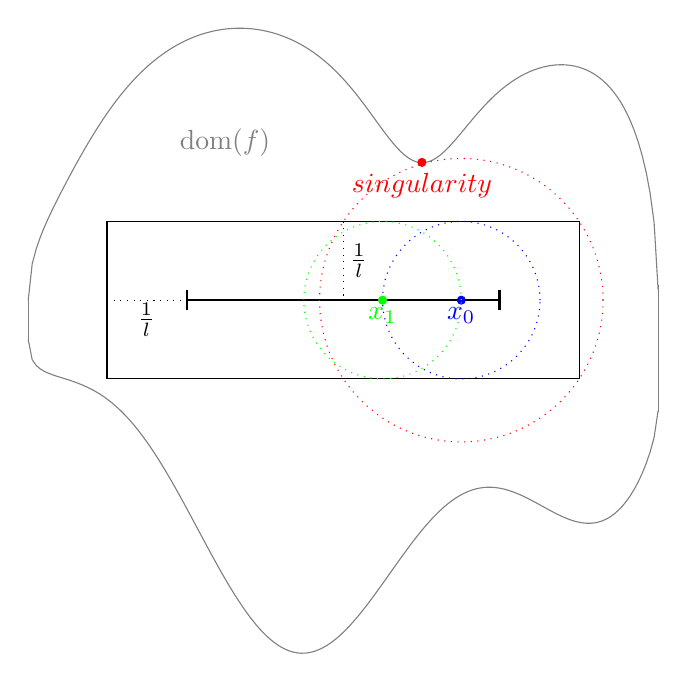
\begin{tikzpicture}
	\draw (-1,1) rectangle (5,-1);
	\draw [thick,|-|] (0,0) -- (4,0);
	\node at (-.5,-.25) {$\frac 1l$};
	\draw [dotted] (-1,0) -- (0,0);
	\node at (2.2,.5) {$\frac 1l$};
	\draw [dotted] (2,1) -- (2,0);
	\draw [domain = 0:8,color=gray] plot[samples=160] (\x-2, {sqrt(16-(\x-4)^2)*(1-1/(\x^2+1) + sin(\x) + (\x/7)^5-\x/6 +1.5- 1/((\x-5)^2+1))/2});
	\draw [domain = 0:8,color=gray] plot[samples=160] (\x-2, {1/(\x^2+1)/2 + sin(80*\x) + (\x/7)^5-\x/6 -1-sqrt(16-(\x-4)^2)/2});
	\draw [color=gray] (-2,0) -- (-2,-.5);
	\draw [color=gray] (6,.19) -- (6,-1.42);
	\node [color=gray] at (.5,2) {$\dom(f)$};
	\draw [fill=blue,radius =.05,color=blue] (3.5,0) circle;
	\node [color=blue] at (3.5,-.2) {$x_0$};
	\draw [radius = 1,color=blue, dotted] (3.5,0) circle;
	\draw [radius = 1.8, color = red, dotted] (3.5,0) circle; 
	\draw [fill=red,radius = .05,color = red] (3,1.75) circle;
	\node [color=red] at (3,1.45) {$singularity$};
	\draw [radius = 1, color = green, dotted] (2.5,0) circle;
	\draw [fill=green, radius = .05, color = green] (2.5,0) circle;
	\node [color=green] at (2.5,-.2) {$x_1$};
\end{tikzpicture}
\end{center}
\caption{A picture of the described situation}
\label{fig:rect}
\end{figure}

To compute the Taylor series around some point of the domain, we use the interpolation procedure described in \cite{Mueller87}:
Computing the coefficient $a_m := \frac{1}{m!}f^{(m)}(x_1)$ can be done by a interpolating $f$ with a polynomial $P$ and compute the derivative $P^{(k)}(x_1)$. 
If $P$ is the unique polynomial interpolating $f$ at $j+1$ points for any $m \leq j$ the error made when computing $a_m$ through $P$ can be approximated by  
\[ \left|a_m - \frac{1}{m!}P^{(k)}(0)\right| \leq M\varepsilon^{j+1-m}4^\frac{4^{j+1}}{\gamma^{m+1}} \]
with $0 < \gamma < R \text{ and } M := \max \{|f(t)|\,:\, |t| = \gamma\}$.
The interpolation is done by partitioning the domain into equidistant points $z_0$, \ldots, $z_{2m+1}$ with distance $h$ and using the Lagrange Interpolation Formula  
\[ P(z) = \sum_{i=0}^{2m} f(z_i) L_{m,i}(z) \text{ with } L_{k,i} = \prod_{0 \leq j \leq 2m \atop j \neq i} \frac{z-z_j}{z_i-z_j}. \]
It follows that 
\[ a_m = \sum_{i=0}^{2m} f(z_i)\frac{h^{-m}l_{m,i}}{i!(2m-i)!} \]
with coefficients $l_{m,i}$ that can be computed in time polynomial in $m$. 

\small

\bibliography{bib}{}
\end{document}